\begin{center}
\begin{tikzpicture}
    \node[anchor=south west,inner sep=0] (image)  at (0,0) {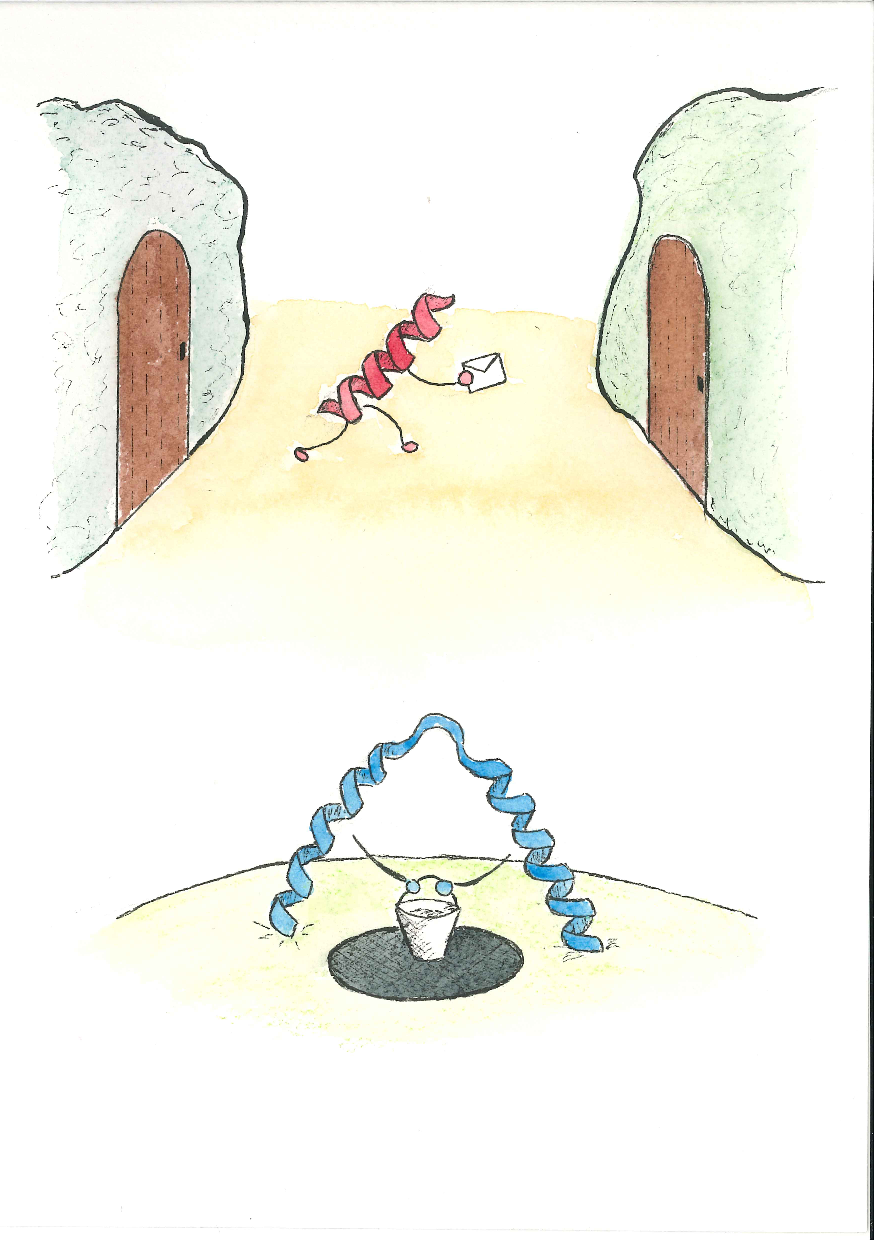
\includegraphics[trim={2mm, 2mm, 2mm, 2mm},width=0.995\pagewidth]{scans/panel-5.pdf}};
    
    
    \begin{scope}[x={(image.south east)},y={(image.north west)}]
        \if\helplines1
        	\draw[help lines,xstep=.1,ystep=.1] (0,0) grid (\N,\N);
        \else
        	\path[help lines,xstep=.1,ystep=.1] (0,0) grid (\N,\N);
        \fi
        \node[align=center, anchor=north, text width=0.3\paperwidth](en1) at (0.5, 0.95) {\english{They perform a variety of tasks, from sending signals to other cells}};
        
        \node[align=center, anchor=north, text width=0.3\paperwidth, below=3mm of en1] {\spanish{Realizan una gran variedad de funciones, desde transmitir señales }};
        
        % %
        \node[align=center, anchor=north, text width=0.3\paperwidth] at (0.2, 0.4) {\english{to pumping water and substances in and out of the cell.}};
        
        \node[align=center, anchor=north, text width=0.3\paperwidth] at (0.8, 0.4) {\spanish{a bombear agua y substancias dentro y fuera de la célula.}};
               
    \end{scope}
    
\end{tikzpicture}
\end{center}

